\chapter{Análisis}

	\noindent En este capítulo se presentará una breve descripción acerca del trabajo terminal haciendo mención del trabajo que se realizó, los problemas que se enfrentaron, así como lo que se logró. Continuando con el capítulo se presentan las Reglas de Negocio y las Reglas del Sistema donde se menciona que es lo que puede realizar la aplicación y que no.\\
	De manera breve  se hace mención de los casos de uso que se realizaron haciendo referencia al apartado Anexos para una consulta más detallada de cada uno de estos.\\
	Así mismo se menciona los Requisitos del usuario, Requisitos funcionales de la aplicación web y Requisitos no funcionales de la aplicación web.\\
	Finalmente se menciona las iteraciones programadas, detallando las actividades realizadas, problemas, logros y si fue necesario, investigación para lograr las metas propuestas.\\
	
	%Agregar etiqueta de diagrama de propuesto
	
	%=========================================================
	%                                                         Prototipo RIDESCOM
	%=========================================================
	\section{Prototipo para el Registro a Interpolit\'ecnicos Deportivos (RIDESCOM)}
	
	\noindent En este capítulo se muestran las iteraciones que realizamos los primeros 4 meses del año 2019 siguiendo la metodología Scrum. En las primeras iteraciones se realizó la investigación acerca de los aspectos fundamentales de las páginas web, con el finn de comprender los conceptos del desarrollo de aplicaciones y poder llevarlos a la práctica. En iteraciones posteriores se hizo un análisis de lo que va a realizar RIDESCOM; de ese análisis se obtuvieron los requisitos funcionales y no funcionales del sistema, una breve descripción de los casos de uso, así como la identificación de los actores, se fueron obteniendo reglas de negocio. Además, de seguir con la investigación y práctica de la creación de aplicaciones web y del uso o implementación de un crawler. Posteriormente se comenzó con la redacción de la documentación técnica, la investigación del estado del arte, el análisis y diseño de la base de datos, la comprensión de comandos de LaTeX, el diseño que tendrá la aplicación, se realizaron pantallas de como lucirá la apliación, se definieron los iconos que se utilizarán en la aplicación, se definieron las tecnologías a utilizar, se implementó un servidor local para la interacción con la aplicación móvil, se creó un primer prototipo de la aplicación con la vista del crawler (Inicio Sesión) y se realizó la redacción de este documento que es el reporte de actividades realizadas. También se creó el repositorio para el desarrollo colaborativo de los documentos. En estas iteraciones surgieron problemas e inconvenientes que afectan al proyecto RIDESCOM tales como la implementación de un crawler, la curva de aprendizaje del desarrollo utilizando Spring MVC, las limitaciones de tiempo debido a que los miembros del equipo trabajan o están realizando su servicio social. Pese a los problemas mencionados o no, tenemos un prototipo funcional de la aplicación así como la mayor parte de la documentación técnica y la elaboración de este documento. El resto de este capítulo presenta en mayor o menor medida los detalles del trabajo realizado en cada iteración.
	
	\section{An\'alisis de factibilidad t\'ecnica}
	
	%=========================================================
	%                                             Requisitos
	%=========================================================
	\section{Reglas de Negocio}
	\noindent La aplicación RIDESCOM permitirá a los alumnos que estén inscritos en el periodo actual, inscribirse en un evento interpolitécnico, consultar los eventos registrados, consultar calendario de eventos. 
	El sistema cuenta con una interfaz que nos permite visualizar las diferentes opciones ofrecidas por el mismo. Para acceder al anterior el usuario debe de tener un usuario y contraseña. Dicho usuario y contraseña, será con el que ingresa al sistema del SAES. 
	Así mismo, habrá “usuarios encargados”, quienes se encargan de controlar y supervisar el uso de éste ante pequeñas porciones de estudiantes (grupos de alumnos). Ahora dichos encargados hay dos tipos el Jefe de Fomento Deportivo, a este se le permitirá crear eventos deportivos, registrar eventos deportivos y restablecer contraseña a los perfiles de los coordinadores. El segundo tipo de encargado es el Coordinador de una Unidad Académica, este podrá registrar los resultados de los participantes en el sistema para poder ser visualizados en la vista principal, podrá generar un reporte de los alumnos registrados durante el periodo que se haya especificado y registrar a los entrenadores que laboran dentro de la Unidad Académica a la que atienda, a continuación se describirán las reglas para cada uno de los actores que se involucran.
	
	\subsection{Reglas de Negocio Jefe de Fomento Deportivo}
	Para que el JFD pueda ingresar a la página RIDESCOM debe de contar con un Usuario y Contraseña, de caso contrario no podrá acceder.
	Una vez dentro de la página de RIDESCOM se le mostrarán las opciones que tiene permitidas, tales como: Evento, Coordinadores, Usuarios, Pruebas en estos dos podrá agregar, editar o eliminar. \\
	
	\noindent Para la vista de Evento, la información se le mostrará en la página principal, si hay eventos registrados estos serán mostrados en la tabla correspondiente, sino se cuenta con datos se mostrará en la tabla el mensaje de que no existen datos.  Para poder agregar un evento se deben de cumplir con algunos campos que son requisito sino se completan los campos no podrá registrar el evento.  Dentro del formulario para crear el evento se debe asignar una fecha en la que los alumnos podrán inscribirse para esto, no debe de ser mayor  a 5 días en la que se realizará el evento. También se debe considerar que no se puede asignar una fecha menor respecto a la fecha en que se está creando el evento. Una vez tenga el evento registrado podrá editar información respecto a este, teniendo en cuenta los campos que son requisito, o en caso contrario eliminar el evento.\\
	
	\noindent Para la vista de Coordinadores, se mostrará la información en una tabla dentro de la página principal, en caso de no contar con datos registrados se mostrará un mensaje de que no existen datos. Para poder agregar un Coordinador de Unidad Académica deberá cumplir con campos que son requisitos sino se completan los campos no podrá registrar el coordinador. Una vez tenga el coordinador registrado podrá editar información respecto a este, teniendo en cuenta los campos que son requisito, o en caso contrario eliminar los datos del coordinador. \\
	
	\noindent Contará con un apartado en el que visualizará los resultados obtenidos por los participantes estos estarán disponibles hasta que concluyan los eventos interpolitécnios y para el JFD solo será de consulta. \\
	
	Para la vista de Pruebas, se mostrará una tabla en la que podrá ver las pruebas registradas, en caso de no tener datos que mostrar se mostrará un mensaje en el que se indique que no hay datos por mostrar. Se podrá agregar pruebas, para ello deberá de cumplir con los campos que son requisitos. De igual manera tendrá campos que son requisito para poder guardar los datos. Una vez guardado las Pruebas podrá editar o eliminar la información. \\
	
	\subsection{Reglas de Negocio Coordinador de Unidad Académica}
	Para que el Coordinador de Unidad Académica pueda ingresar a la página RIDESCOM debe de contar con un Usuario y Contraseña, de caso contrario no podrá acceder.\\
	
	Una vez dentro de la página de RIDESCOM se le mostrarán las opciones que tiene permitidas, tales como: Constancias, Calendario, Resultados, Consulta Inscritos, DIfundir Evento y Entrenadores. Las vistas antes mencionadas exceptuando Resultados y Difundir Evento, serán vistas de solo lectura.\\
	
	Para la vista de Constancias el Coordinador de la Unidad Académica podrá consultar si el alumno participó en un evento para que posteriormente, él pueda comenzar el trámite correspondiente para la generación de la constancia. Será solo vista de consulta/lectura.\\
	
	Para la vista de Calendario, se mostrará en la página principal del Coordinador una tabla con los datos que le corresponden, en caso de no tener información se mostrará el mensaje de que no existen datos. Esta vista sólo será de lectura.\\
	
	Para la vista de Resultados el Coordinador de la Unidad Académica podrá visualizar la información en una tabla dentro de la página principal, en caso de no tener datos se mostrará el mensaje de que no existen datos Para ingresar los resultados obtenidos de los participantes, como el tiempo que se obtuvo, el lugar, etc., deberá de llenar los campos que son requisitos, sino se completan los campos no podrá registrarse el evento. Una vez que se tengan los datos registrados podrá editar o eliminar estos.\\
	
	Para la vista Difundir Evento, el Coordinador de la Unidad Académica podrá visualizar los eventos que han sido registrados, al selecciona la opción difundir se le mostrará la opción de difundirlo en la red social de facebook.\\
	
	Para la vista de Entrenadores, se mostrará la información dentro de la vista principal en una tabla, en caso de no contar con información se mostrará el mensaje de que no existen datos. Para agregar datos de un Entrenador se deben de cumplir con datos que son requisitos. Una vez que se tengan datos registrados podrá editar o eliminar la información. \\
	
	\subsection{Reglas de Negocio Alumno}
	Para que el alumno pueda ingresar a la página RIDESCOM debe de contar con un Usuario y Contraseña, de caso contrario no podrá acceder.\\
	
	Una vez dentro de la página de RIDESCOM se le mostrarán las opciones que tiene permitidas, tales como: Calendario, Inscribe Interpolitecnico, Historial,  Resultados, Eventos Inscritos. Las vistas antes mencionadas serán solo lectura exeptuando la vista de INscribe Interpolitecnico.\\
	
	Para la vista de Calendario se mostrará en la página principal en una tabla que contenga la información, en caso de que esta no cuente con información se mostrará el mensaje de que no existen datos. Esta vista sólo será de lectura para el alumno.\\
	
	Para la vista de Inscribir Interpolitecnio, el alumno pueda inscribir un Evento Interpolitecnico deberá como primer punto, validar su status académico, para ello se le mostrará en segunda ocasión el inicio de sesión con esto, se verificará su estatus académico. Si el alumno está inscrito entonces se le mostrará una segundo vista en la que solo será de lectura y verificará si sus datos son correctos. En caso de que el alumno no esté inscrito se le mostrará un mensaje para notificarle que no puede inscribirse dado que no está inscrito en el periodo actual. \\
	Si la información que se le presenta es correcta podrá continuar para seleccionar el evento en el que desea participar y así concluir con su inscripción. \\
	
	Para la vista Historial, se mostrará al alumno una tabla que le proporcione información de los eventos en los que ha participado a lo largo de su trayectoria académica. Esta vista es de solo lectura.\\
	
	Para la vista Resultado, se mostrará la información de los resultados del último evento en el que a participado. Esta vista es de solo lectura.\\
	
	Para la vista de Eventos Inscritos, mostrará el o los eventos a los que se a registrado el alumno en el periodo en curso. Esta vista es de solo lectura.\\
	
	\noindent A continuación se mostrará en una tabla un resumen de las Reglas de Negocio de cada uno de los actores.
	
	\begin{table}[hbt!]
		\begin{center}
			\begin{tabular}{|p{30mm}|p{100mm}|}
				\hline
				\multicolumn{2}{|c|}{Jefe de Fomento Deportivo} \\
				\hline
				Identificador & Descripción \\
				\hline 
				RN 1 & Para ingresar a la página debe de contar con un usuario y contraseña. \\ \hline
				RN 2 &  Para registrar un nuevo evento deben de completarse todos los campos que son requisito.\\ \hline
				RN 3 & Para registrar un evento debe de considerar que la fecha de este no sea menor a la fecha en la que se quiere realizar el mismo (no debe de ser mayor  a 5 días en la que se realizará el evento). \\ \hline
				RN 4 &  La fecha de inicio de registro para los alumnos no rebase la fecha en la que se realizará el evento.\\ \hline
				RN 5 &  La fecha de fin de registro para los alumnos no rebase la fecha en la que se realizará el evento. \\ \hline
				RN 6 & Para editar los datos de un evento, no debe de haber alumnos inscritos. \\ \hline
				RN 7 &  Al editar los datos de un evento debe considerar completar todos los campos.\\ \hline
				RN 8 &  Para eliminar un evento, no debe de haber alumnos inscritos en este.\\ \hline
				RN 9 &  Para agregar un deporte, todos los campos que son requisito deben completarse.\\ \hline
				RN 10 &  Al editar un deporte, se debe considerar completar todos los campos requeridos.\\ \hline
				RN 11 &  Para registrar una Prueba, se debe de completar todos los campos.\\ \hline
				RN 12 & Al editar los datos se debe considerar completar todos los campos.\\ \hline
				RN 13 &  Al registrar un nuevo Coordinador, se debe asignar un usuario y contraseña.\\ \hline
				RN 14 &  Para completar el registro, debe completarse todos los campos requeridos.\\ \hline
				RN 15 &  Al editar los datos de un Coordinador, se debe tomar en cuenta completar todos los campos requeridos.\\ \hline
				RN 16 &  Para registrar una Sede, deben completarse todos los campos requeridos.\\ \hline
				RN 17 &  Al editar los datos de una Sede, se debe considerar que esta no esté asignada en un evento.\\ \hline
			\end{tabular}
			\caption{Reglas de Negocio Jefe de Fomento Deportivo.}
			\label{RNJFD}
		\end{center}
	\end{table}
	
	\begin{table}[hbt!]
		\begin{center}
			\begin{tabular}{|p{30mm}|p{100mm}|}
				\hline
				\multicolumn{2}{|c|}{Coordinador de Unidad Acedémica} \\
				\hline
				Identificador & Descripción \\
				\hline 
				RN 18 &  Para ingresar a la página debe de contar con un usuario y contraseña.\\ \hline
				RN 19 & Las credenciales deben estar activas y ser proporcionadas por el Jefe de Fomento Deportivo.\\ \hline
				RN 20 & Para ingresar los resultados, debe seleccionar un usuario. \\ \hline
				RN 21 & Se debe seleccionar una prueba correspondiente al alumno.\\ \hline
				RN 22 & Para terminar el proceso de registro de resultados, debe completar los campos requeridos. \\ \hline
				RN 23 & Para registrar un entrenador debe llenar todos los campos requeridos.\\ \hline
				RN 24 & Para obtener la cédula de inscripción, el coordinador deberá de seleccionar el tipo de deporte, así como el ciclo escolar. \\ \hline
				RN 25 & Para consultar si un alumno participó en un evento, se debe buscar por medio de su boleta o por el ciclo escolar en el que participó.\\ \hline
				RN 26 & Para difundir un evento, deberá seleccionar el evento de la tabla y seleccionar el medio por el cual quiere compartir el evento.\\ \hline
			\end{tabular}
			\caption{Reglas de Negocio Coordinador de Unidad Académicas.}
			\label{RNCUA}
		\end{center}
	\end{table}
	
	\pagebreak
	
	\begin{table}[hbt!]
		\begin{center}
			\begin{tabular}{|p{30mm}|p{100mm}|}
				\hline
				\multicolumn{2}{|c|}{Alumno} \\ \hline
				Identificador & Descripción \\ \hline 
				RN & Para ingresar a la página debe de contar con un usuario y contraseña.\\ \hline
				RN & El alumno debe verificar el estatus académico para poder registrarse en un evento.\\ \hline
				RN & Para concluir el registro al evento, debe de llenar todos los campos requeridos.\\ \hline
				RN & Puede inscribirse en los eventos que desee, siempre y cuando no tenga traslape en horas de los eventos.\\ \hline
				RN & \\ \hline
				RN & \\ \hline
			\end{tabular}
			\caption{Reglas de Negocio para el alumno.}
			\label{RNA}
		\end{center}
	\end{table}
	
	
	%=========================================================
	%                                             Requisitos
	%=========================================================
	\section{Reglas del Sistema}
	\noindent El alumno que desee participar en un evento interpolitécnico hará uso de la aplicación web RIDESCOM. Como primer punto deberá iniciar sesión en la misma, ingresando el usuario y contraseña con el que entra a sistema SAES (Sistema de Administración Escolar). Si los datos ingresados son correctos, se le dará acceso a la aplicación RIDESCOM, en caso contrario no se le dará acceso para poder registrarse en un evento. Sin embargo, podrá seguir visualizando datos generales, como lo es el calendario de eventos, resultados de eventos y los eventos que se practican dentro de la unidad académica.
	El Jefe de Fomento Deportivo podrá dar de alta a un Coordinador de alguna Unidad Académica. Para dar de alta un evento deportivo deberá llenar todos los campos requeridos, tendrá la opción de agregar una descripción si así lo desea. 
	El Coordinador de la Unidad Académica registrará a los entrenadores de las actividades deportivas deberá llenar los campos requeridos para poder concluir el registro. En caso de que exista un entrenador ya haya sido registrado, la aplicación le notificará. Una vez concluido los eventos deportivos, este registrará los resultados obtenidos por los participantes para que puedan ser vistos por la comunidad en general.
	
	
	%=========================================================
	%                                            Casos de Uso
	%=========================================================
	\section{Casos de Uso}
		\subsection{CU1 Iniciar Sesión}
		\noindent En este caso de uso se describe el funcionamiento del módulo Iniciar sesión para el alumno. Se describe paso a paso la trayectoria, asi como los posibles errores que pueden existir. Para mas detalles consulta el apartado Anexos en la sección D CU \ref{CU1_Iniciarsesion}.
		
		\subsection{CU2 Inscribir a un evento interpolitécnico deportivo}
		\noindent En este caso de uso se describe el funcionamiento del módulo Inscribir a un evento interpolitécnico deportivo. Se describe paso a paso la trayectoria, asi como los posibles errores que pueden existir. Para mas detalles consulta el apartado Anexos en la sección D CU \ref{CU2_Inscribirauneventointerpolitécnicodeportivo}
		
		\subsection{CU 2.1 Validación estatus académico}
		\noindent En este caso de uso se describe el funcionamiento del módulo validación de estatus académico. Se describe paso a paso la trayectoria, asi como los posibles errores que pueden existir. Para mas detalles consulta el apartado Anexos en la sección D CU  \ref{CU3_Validacionestatusacademico}
		
		\subsection{Registro}
		\noindent En este caso de uso se omitió para el desarrollo del proyecto ya que el registro ya no será requerido en el sistema, sin embargo se muestra como evidencia del trabajo realizado, este describe el funcionamiento del módulo registro para los alumnos. Se describe paso a paso la trayectoria, asi como los posibles errores que pueden existir. Para mas detalles consulta el apartado Anexos en la sección D CU \ref{CU_Registro}
		
		\subsection{Validación de perfil}
		\noindent En este caso de uso se omitió para el desarrollo del proyecto ya que el registro ya no será requerido en el sistema, sin embargo se muestra como evidencia del trabajo realizado, este describe el funcionamiento del módulo validación del perfil. Se describe paso a paso la trayectoria, asi como los posibles errores que pueden existir. Para mas detalles consulta el apartado Anexos en la sección D CU \ref{CU_Validacionperfil}
	
	
	
	%=========================================================
	%                                                         Requisitos de interaccion con el usuario
	%=========================================================
	\section{Requisitos del usuario}
	\begin{table}[htbp]
		\begin{center}
			\begin{tabular}{|l|p{45mm}|p{45mm}|p{45mm}|l}
				\hline
				Id & Nombre & Descripción & Prioridad \\
				\hline 
				RF1 & Registro de eventos & En la aplicación web se podrán registrar, modificar, eliminar y consultar  en un formulario todos los datos para identificar un evento.
				& MEDIA \\ \hline
				RF2 & Registro de participantes & En la aplicación web se podrán registrar, modificar, eliminar y consultar  en un formulario los datos del participante & ALTA  \\ \hline
				RF3 & Vista al público & En una pantalla se mostrarán los participantes que estén registrados en la aplicación y ver sus resultados de competencia. & MEDIO \\ \hline
				RF4 & Conexión con red social FACEBOOK. & Gracias a los datos que identifican a un evento se podrá promover en la red social FACEBOOK mediante el uso de API.& ALTA \\ \hline
				RF5 & Realizar una interfaz para los participantes (alumnos). &Se creará un(una ventana)  sitio para los alumnos que quieran participar en algún evento deportivo(, haciendo su registro, consultar estatus). & MEDIA \\ \hline
				RF6 & Mostrar una tabla de estadísticas. & En una pantalla (vista)  se mostrará todas las áreas deportivas que participaron en el evento deportivo y  número de participantes. & ALTA \\ \hline
				RF7 & Registrar un coordinador & El coordinador que utilizará la aplicación web tendrá que ser registrado en la base de datos. & ALTA \\ \hline
				RF8 & Vista para el coordinador. &El coordinador tendrá una vista donde podrá dar de alta eventos, participantes y generar cédulas de inscripción. & MEDIA \\ \hline
				RF9  & Historial & Para que se tenga un monitoreo de participantes. & ALTA \\ \hline
			\end{tabular}
			\caption{Requerimientos del Usuario.}
			\label{tabla:sencilla}
		\end{center}
	\end{table}
	\pagebreak
	
	%=========================================================
	%                                                         Requisitos funcionales
	%=========================================================
	\section{Requisitos funcionales de la aplicación web}
	
	\begin{table}[htbp]
		\begin{center}
			\begin{tabular}{|l|p{45mm}|p{45mm}|p{45mm}|l}
				\hline
				Id & Nombre & Descripción & Prioridad \\
				\hline 
				RF1 & Validación de datos de los participantes. & La aplicación contará con un mecanismo de comprobación de estado académico (inscrito). & ALTA \\ \hline
				RF2 & Historial de participante. & Para tener seguimiento del participante durante su trayectoria académica & MEDIA  \\ \hline
				RF3 & Comunicación con la red social FACEBOOK &Habrá comunicación con la red social FACEBOOK para la publicación de eventos registrados en la aplicación.  & MEDIO \\ \hline
				RF4 & Creación de perfiles. & Se podrá asignar un perfil a un usuario.& MEDIA \\ \hline
			\end{tabular}
			\pagebreak
			\caption{Requerimientos funcionales de la aplicación web.}
			\label{tabla:sencilla}
		\end{center}
	\end{table}
	
	
	%=========================================================
	%                                                         Requisitos de informacion
	%=========================================================
	\section{Requisitos no funcionales de la aplicación web}
	
	\begin{table}[htbp]
		\begin{center}
			\begin{tabular}{|l|p{45mm}|p{45mm}|p{45mm}|l}
				\hline
				Id & Nombre & Descripción & Prioridad \\
				\hline 
				RF1 & Vista de consulta genera. & Comunidad ajena a los participantes podrán ver los resultados. & MEDIA \\ \hline
				RF2 & Lista de registros &El usuario podrá consultar sus registros realizados & MEDIA   \\ \hline
				RF3 & Recuperación de contraseña &El usuario participante podrá recuperar su contraseña. & MEDIO \\ \hline
			\end{tabular}
			\caption{Requerimientos no funcionales de la aplicación web.}
			\label{tabla:sencilla}
		\end{center}
	\end{table}
	
	
	%=========================================================
	%                                                         Reglas de Negocio del Sistema
	%=========================================================
	%\section{Reglas de necocio de la aplicación}
	

	\section{MockUp}
	\noindent Las vistas han cambiado conforme avanza el proyecto, en este caso, se han omitido unas vistas ya que durante nuestra investigación para implementar el registro a la página RIDESCOM para los alumnos, en un inicio se planteo hacer una conexión con la base de datos de la Dirección de Administración Escolera (DAE) para poder verificar que sus datos sean reales. Este método de comprobación iba a ser difícil de llevar a cabo ya que por el hecho de manejar datos sensibles no se nos podía ser brindada. Por esta razón se investigo como poder implementar un crawler, que se conecta con el SAES. Dentro de la página RIDESCOM se solicitan los mismos campos que en el SAES: Usuario, Contraseña y Captcha, si los datos que se ingresaron son correctos el alumno podrá ingresar a RIDESCOM, en caso contrario se le notificará que los datos son erróneos. \\
	Las vistas que se eliminaron son las siguientes: 
	
	\begin{figure}[hbt!]
		\centering
		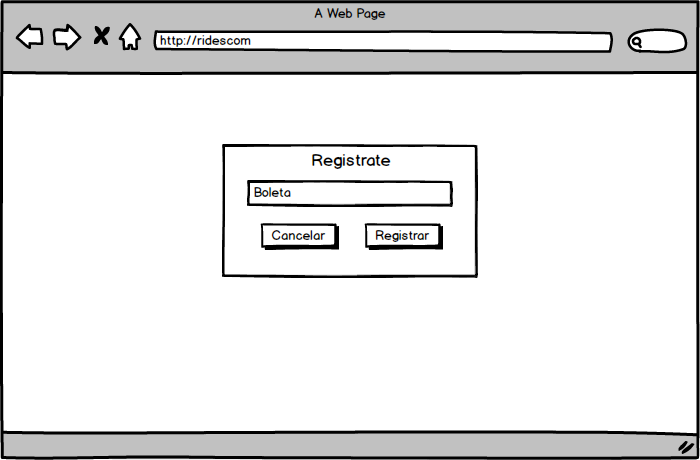
\includegraphics[width=10cm, height=6cm]{Imagenes/Disenos/VistasBorradas/p1_Registro.png}
		\caption{Registro para los alumnos.}
	\end{figure}
	
	\begin{figure}[hbt!]
		\centering
		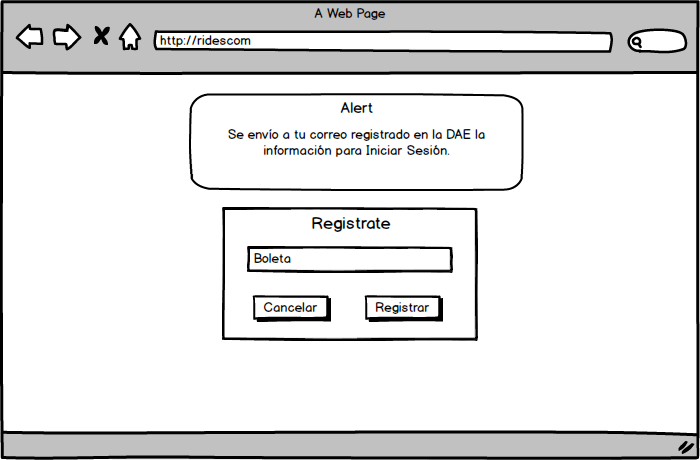
\includegraphics[width=10cm, height=6cm]{Imagenes/Disenos/VistasBorradas/ConfirmacionRegistro.png}
		\caption{Confirmación registro para los alumnos.}
	\end{figure}
	
	\begin{figure}[hbt!]
		\centering
		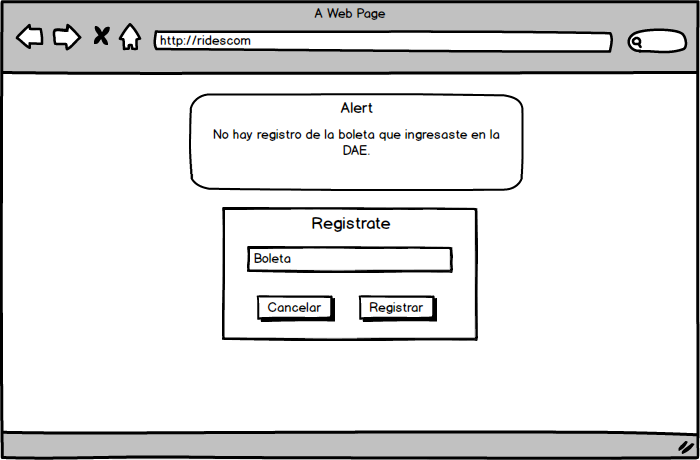
\includegraphics[width=10cm, height=6cm]{Imagenes/Disenos/VistasBorradas/p3RechazoRegistro.png}
		\caption{Rechazo registro para los alumnos.}
	\end{figure}

	\begin{figure}[hbt!]
		\centering
		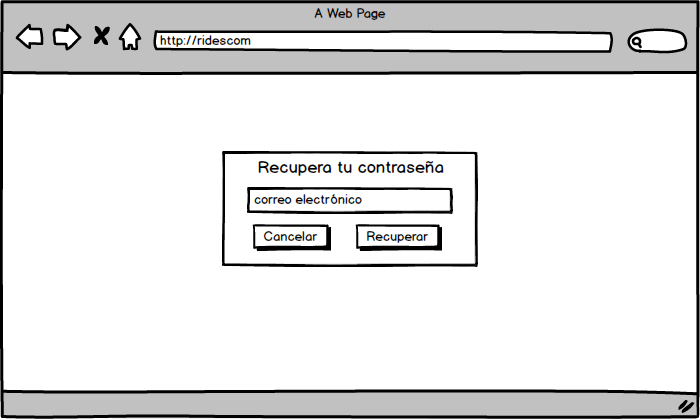
\includegraphics[width=10cm, height=6cm]{Imagenes/Disenos/VistasBorradas/p5Recuperarcontrasena.png}
		\caption{Recuperar contraseña para los alumnos.}
	\end{figure}

	\begin{figure}[hbt!]
		\centering
		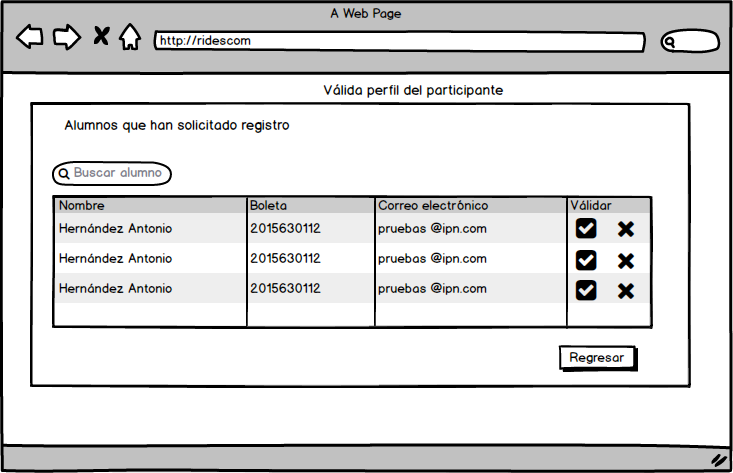
\includegraphics[width=10cm, height=6cm]{Imagenes/Disenos/VistasBorradas/p18ValidaPerfil.png}
		\caption{Validar perfil de los alumnos.}
	\end{figure}
	\pagebreak

	